% Generated by Sphinx.
\def\sphinxdocclass{report}
\documentclass[letterpaper,10pt,english]{sphinxmanual}
\usepackage[utf8]{inputenc}
\DeclareUnicodeCharacter{00A0}{\nobreakspace}
\usepackage{cmap}
\usepackage[T1]{fontenc}
\usepackage{babel}
\usepackage{times}
\usepackage[Bjarne]{fncychap}
\usepackage{longtable}
\usepackage{sphinx}
\usepackage{multirow}


\title{OpenStack Trove plugin for Fuel Documentation}
\date{August 16, 2016}
\release{1.0-1.0.3-1}
\author{AT\&T Services, Inc.}
\newcommand{\sphinxlogo}{}
\renewcommand{\releasename}{Release}
\makeindex

\makeatletter
\def\PYG@reset{\let\PYG@it=\relax \let\PYG@bf=\relax%
    \let\PYG@ul=\relax \let\PYG@tc=\relax%
    \let\PYG@bc=\relax \let\PYG@ff=\relax}
\def\PYG@tok#1{\csname PYG@tok@#1\endcsname}
\def\PYG@toks#1+{\ifx\relax#1\empty\else%
    \PYG@tok{#1}\expandafter\PYG@toks\fi}
\def\PYG@do#1{\PYG@bc{\PYG@tc{\PYG@ul{%
    \PYG@it{\PYG@bf{\PYG@ff{#1}}}}}}}
\def\PYG#1#2{\PYG@reset\PYG@toks#1+\relax+\PYG@do{#2}}

\expandafter\def\csname PYG@tok@gd\endcsname{\def\PYG@tc##1{\textcolor[rgb]{0.63,0.00,0.00}{##1}}}
\expandafter\def\csname PYG@tok@gu\endcsname{\let\PYG@bf=\textbf\def\PYG@tc##1{\textcolor[rgb]{0.50,0.00,0.50}{##1}}}
\expandafter\def\csname PYG@tok@gt\endcsname{\def\PYG@tc##1{\textcolor[rgb]{0.00,0.27,0.87}{##1}}}
\expandafter\def\csname PYG@tok@gs\endcsname{\let\PYG@bf=\textbf}
\expandafter\def\csname PYG@tok@gr\endcsname{\def\PYG@tc##1{\textcolor[rgb]{1.00,0.00,0.00}{##1}}}
\expandafter\def\csname PYG@tok@cm\endcsname{\let\PYG@it=\textit\def\PYG@tc##1{\textcolor[rgb]{0.25,0.50,0.56}{##1}}}
\expandafter\def\csname PYG@tok@vg\endcsname{\def\PYG@tc##1{\textcolor[rgb]{0.73,0.38,0.84}{##1}}}
\expandafter\def\csname PYG@tok@vi\endcsname{\def\PYG@tc##1{\textcolor[rgb]{0.73,0.38,0.84}{##1}}}
\expandafter\def\csname PYG@tok@mh\endcsname{\def\PYG@tc##1{\textcolor[rgb]{0.13,0.50,0.31}{##1}}}
\expandafter\def\csname PYG@tok@cs\endcsname{\def\PYG@tc##1{\textcolor[rgb]{0.25,0.50,0.56}{##1}}\def\PYG@bc##1{\setlength{\fboxsep}{0pt}\colorbox[rgb]{1.00,0.94,0.94}{\strut ##1}}}
\expandafter\def\csname PYG@tok@ge\endcsname{\let\PYG@it=\textit}
\expandafter\def\csname PYG@tok@vc\endcsname{\def\PYG@tc##1{\textcolor[rgb]{0.73,0.38,0.84}{##1}}}
\expandafter\def\csname PYG@tok@il\endcsname{\def\PYG@tc##1{\textcolor[rgb]{0.13,0.50,0.31}{##1}}}
\expandafter\def\csname PYG@tok@go\endcsname{\def\PYG@tc##1{\textcolor[rgb]{0.20,0.20,0.20}{##1}}}
\expandafter\def\csname PYG@tok@cp\endcsname{\def\PYG@tc##1{\textcolor[rgb]{0.00,0.44,0.13}{##1}}}
\expandafter\def\csname PYG@tok@gi\endcsname{\def\PYG@tc##1{\textcolor[rgb]{0.00,0.63,0.00}{##1}}}
\expandafter\def\csname PYG@tok@gh\endcsname{\let\PYG@bf=\textbf\def\PYG@tc##1{\textcolor[rgb]{0.00,0.00,0.50}{##1}}}
\expandafter\def\csname PYG@tok@ni\endcsname{\let\PYG@bf=\textbf\def\PYG@tc##1{\textcolor[rgb]{0.84,0.33,0.22}{##1}}}
\expandafter\def\csname PYG@tok@nl\endcsname{\let\PYG@bf=\textbf\def\PYG@tc##1{\textcolor[rgb]{0.00,0.13,0.44}{##1}}}
\expandafter\def\csname PYG@tok@nn\endcsname{\let\PYG@bf=\textbf\def\PYG@tc##1{\textcolor[rgb]{0.05,0.52,0.71}{##1}}}
\expandafter\def\csname PYG@tok@no\endcsname{\def\PYG@tc##1{\textcolor[rgb]{0.38,0.68,0.84}{##1}}}
\expandafter\def\csname PYG@tok@na\endcsname{\def\PYG@tc##1{\textcolor[rgb]{0.25,0.44,0.63}{##1}}}
\expandafter\def\csname PYG@tok@nb\endcsname{\def\PYG@tc##1{\textcolor[rgb]{0.00,0.44,0.13}{##1}}}
\expandafter\def\csname PYG@tok@nc\endcsname{\let\PYG@bf=\textbf\def\PYG@tc##1{\textcolor[rgb]{0.05,0.52,0.71}{##1}}}
\expandafter\def\csname PYG@tok@nd\endcsname{\let\PYG@bf=\textbf\def\PYG@tc##1{\textcolor[rgb]{0.33,0.33,0.33}{##1}}}
\expandafter\def\csname PYG@tok@ne\endcsname{\def\PYG@tc##1{\textcolor[rgb]{0.00,0.44,0.13}{##1}}}
\expandafter\def\csname PYG@tok@nf\endcsname{\def\PYG@tc##1{\textcolor[rgb]{0.02,0.16,0.49}{##1}}}
\expandafter\def\csname PYG@tok@si\endcsname{\let\PYG@it=\textit\def\PYG@tc##1{\textcolor[rgb]{0.44,0.63,0.82}{##1}}}
\expandafter\def\csname PYG@tok@s2\endcsname{\def\PYG@tc##1{\textcolor[rgb]{0.25,0.44,0.63}{##1}}}
\expandafter\def\csname PYG@tok@nt\endcsname{\let\PYG@bf=\textbf\def\PYG@tc##1{\textcolor[rgb]{0.02,0.16,0.45}{##1}}}
\expandafter\def\csname PYG@tok@nv\endcsname{\def\PYG@tc##1{\textcolor[rgb]{0.73,0.38,0.84}{##1}}}
\expandafter\def\csname PYG@tok@s1\endcsname{\def\PYG@tc##1{\textcolor[rgb]{0.25,0.44,0.63}{##1}}}
\expandafter\def\csname PYG@tok@ch\endcsname{\let\PYG@it=\textit\def\PYG@tc##1{\textcolor[rgb]{0.25,0.50,0.56}{##1}}}
\expandafter\def\csname PYG@tok@m\endcsname{\def\PYG@tc##1{\textcolor[rgb]{0.13,0.50,0.31}{##1}}}
\expandafter\def\csname PYG@tok@gp\endcsname{\let\PYG@bf=\textbf\def\PYG@tc##1{\textcolor[rgb]{0.78,0.36,0.04}{##1}}}
\expandafter\def\csname PYG@tok@sh\endcsname{\def\PYG@tc##1{\textcolor[rgb]{0.25,0.44,0.63}{##1}}}
\expandafter\def\csname PYG@tok@ow\endcsname{\let\PYG@bf=\textbf\def\PYG@tc##1{\textcolor[rgb]{0.00,0.44,0.13}{##1}}}
\expandafter\def\csname PYG@tok@sx\endcsname{\def\PYG@tc##1{\textcolor[rgb]{0.78,0.36,0.04}{##1}}}
\expandafter\def\csname PYG@tok@bp\endcsname{\def\PYG@tc##1{\textcolor[rgb]{0.00,0.44,0.13}{##1}}}
\expandafter\def\csname PYG@tok@c1\endcsname{\let\PYG@it=\textit\def\PYG@tc##1{\textcolor[rgb]{0.25,0.50,0.56}{##1}}}
\expandafter\def\csname PYG@tok@o\endcsname{\def\PYG@tc##1{\textcolor[rgb]{0.40,0.40,0.40}{##1}}}
\expandafter\def\csname PYG@tok@kc\endcsname{\let\PYG@bf=\textbf\def\PYG@tc##1{\textcolor[rgb]{0.00,0.44,0.13}{##1}}}
\expandafter\def\csname PYG@tok@c\endcsname{\let\PYG@it=\textit\def\PYG@tc##1{\textcolor[rgb]{0.25,0.50,0.56}{##1}}}
\expandafter\def\csname PYG@tok@mf\endcsname{\def\PYG@tc##1{\textcolor[rgb]{0.13,0.50,0.31}{##1}}}
\expandafter\def\csname PYG@tok@err\endcsname{\def\PYG@bc##1{\setlength{\fboxsep}{0pt}\fcolorbox[rgb]{1.00,0.00,0.00}{1,1,1}{\strut ##1}}}
\expandafter\def\csname PYG@tok@mb\endcsname{\def\PYG@tc##1{\textcolor[rgb]{0.13,0.50,0.31}{##1}}}
\expandafter\def\csname PYG@tok@ss\endcsname{\def\PYG@tc##1{\textcolor[rgb]{0.32,0.47,0.09}{##1}}}
\expandafter\def\csname PYG@tok@sr\endcsname{\def\PYG@tc##1{\textcolor[rgb]{0.14,0.33,0.53}{##1}}}
\expandafter\def\csname PYG@tok@mo\endcsname{\def\PYG@tc##1{\textcolor[rgb]{0.13,0.50,0.31}{##1}}}
\expandafter\def\csname PYG@tok@kd\endcsname{\let\PYG@bf=\textbf\def\PYG@tc##1{\textcolor[rgb]{0.00,0.44,0.13}{##1}}}
\expandafter\def\csname PYG@tok@mi\endcsname{\def\PYG@tc##1{\textcolor[rgb]{0.13,0.50,0.31}{##1}}}
\expandafter\def\csname PYG@tok@kn\endcsname{\let\PYG@bf=\textbf\def\PYG@tc##1{\textcolor[rgb]{0.00,0.44,0.13}{##1}}}
\expandafter\def\csname PYG@tok@cpf\endcsname{\let\PYG@it=\textit\def\PYG@tc##1{\textcolor[rgb]{0.25,0.50,0.56}{##1}}}
\expandafter\def\csname PYG@tok@kr\endcsname{\let\PYG@bf=\textbf\def\PYG@tc##1{\textcolor[rgb]{0.00,0.44,0.13}{##1}}}
\expandafter\def\csname PYG@tok@s\endcsname{\def\PYG@tc##1{\textcolor[rgb]{0.25,0.44,0.63}{##1}}}
\expandafter\def\csname PYG@tok@kp\endcsname{\def\PYG@tc##1{\textcolor[rgb]{0.00,0.44,0.13}{##1}}}
\expandafter\def\csname PYG@tok@w\endcsname{\def\PYG@tc##1{\textcolor[rgb]{0.73,0.73,0.73}{##1}}}
\expandafter\def\csname PYG@tok@kt\endcsname{\def\PYG@tc##1{\textcolor[rgb]{0.56,0.13,0.00}{##1}}}
\expandafter\def\csname PYG@tok@sc\endcsname{\def\PYG@tc##1{\textcolor[rgb]{0.25,0.44,0.63}{##1}}}
\expandafter\def\csname PYG@tok@sb\endcsname{\def\PYG@tc##1{\textcolor[rgb]{0.25,0.44,0.63}{##1}}}
\expandafter\def\csname PYG@tok@k\endcsname{\let\PYG@bf=\textbf\def\PYG@tc##1{\textcolor[rgb]{0.00,0.44,0.13}{##1}}}
\expandafter\def\csname PYG@tok@se\endcsname{\let\PYG@bf=\textbf\def\PYG@tc##1{\textcolor[rgb]{0.25,0.44,0.63}{##1}}}
\expandafter\def\csname PYG@tok@sd\endcsname{\let\PYG@it=\textit\def\PYG@tc##1{\textcolor[rgb]{0.25,0.44,0.63}{##1}}}

\def\PYGZbs{\char`\\}
\def\PYGZus{\char`\_}
\def\PYGZob{\char`\{}
\def\PYGZcb{\char`\}}
\def\PYGZca{\char`\^}
\def\PYGZam{\char`\&}
\def\PYGZlt{\char`\<}
\def\PYGZgt{\char`\>}
\def\PYGZsh{\char`\#}
\def\PYGZpc{\char`\%}
\def\PYGZdl{\char`\$}
\def\PYGZhy{\char`\-}
\def\PYGZsq{\char`\'}
\def\PYGZdq{\char`\"}
\def\PYGZti{\char`\~}
% for compatibility with earlier versions
\def\PYGZat{@}
\def\PYGZlb{[}
\def\PYGZrb{]}
\makeatother

\renewcommand\PYGZsq{\textquotesingle}

\begin{document}

\maketitle
\tableofcontents
\phantomsection\label{index::doc}


Contents:


\chapter{Document purpose}
\label{overview::doc}\label{overview:welcome-to-openstack-trove-plugin-for-fuel-s-documentation}\label{overview:document-purpose}\label{overview:overview}
This document provides instructions for installing, configuring and using
OpenStack Trove plugin for Fuel.


\section{OpenStack Trove plugin}
\label{overview:openstack-trove-plugin}
The OpenStack Trove plugin provides ability to install an OpenStack
environment with Trove deployed on dedicated nodes. Trove provides
scalable and reliable Cloud Database as a Service provisioning functionality
for both relational and non-relational database engines, and to continue to
improve its fully-featured and extensible open source framework.

Plugin is hot-pluggable and It can be enabled in a new environment or existing
deployed environment without the plugin.


\section{Requirements}
\label{overview:requirements}
\begin{tabulary}{\linewidth}{|L|L|}
\hline
\textsf{\relax 
Requirement
} & \textsf{\relax 
Version/Comment
}\\
\hline
Fuel
 & 
8.0 release
\\

OpenStack compatibility
 & 
Liberty
\\

Operating systems
 & 
Ubuntu 14.04 LTS
\\
\hline\end{tabulary}



\section{Limitations}
\label{overview:limitations}
OpenStack Trove plugin deploys a dedicated RabbitMQ Cluster on Trove nodes for
for security reasons.
\href{http://lists.openstack.org/pipermail/openstack-dev/2015-April/061759.html/}{Dedicated RabbitMQ}.

If the OpenStack Trove plugin is enabled for an environment, it is impossible
to assign Trove and Controller roles to the same node.

There is a Detach RabbitMQ plugin, which enable user to install RabbitMQ
on separate nodes. Detach RabbitMQ plugin role should not be used together
with Trove plugin role, User should ensure that:
\begin{itemize}
\item {} 
Trove and RabbitMQ roles shoud not to be assigned to the same nodes

\end{itemize}


\chapter{Installation Guide}
\label{installation_guide:installation}\label{installation_guide::doc}\label{installation_guide:installation-guide}\begin{enumerate}
\item {} 
Start with \href{https://docs.mirantis.com/openstack/fuel/fuel-8.0/fuel-install-guide.html\#introduction-to-fuel-installation}{installing Fuel Master node} \footnote{
\href{https://docs.mirantis.com/openstack/fuel/fuel-8.0/fuel-install-guide.html\#introduction-to-fuel-installation}{https://docs.mirantis.com/openstack/fuel/fuel-8.0/fuel-install-guide.html\#introduction-to-fuel-installation}
}.

\item {} 
Install \href{https://wiki.openstack.org/wiki/Fuel/Plugins\#install\_latest}{Fuel Plugin Builder on Fuel Master node} \footnote{
\href{https://wiki.openstack.org/wiki/Fuel/Plugins\#install\_latest}{https://wiki.openstack.org/wiki/Fuel/Plugins\#install\_latest}
}.

\item {} 
Install Git on Fuel Master node:

\begin{Verbatim}[commandchars=\\\{\}]
[root@fuel \PYGZti{}]\PYGZsh{} yum install git \PYGZhy{}y
\end{Verbatim}

\item {} 
Clone the plugin from \href{http://github.com/openstack/fuel-plugin-dbaas-trove.git}{Github} \footnote{
\href{http://github.com/openstack/fuel-plugin-dbaas-trove.git}{http://github.com/openstack/fuel-plugin-dbaas-trove.git}
}.
\begin{quote}

{[}\href{mailto:root@fuel}{root@fuel} \textasciitilde{}{]}\# git clone \href{http://github.com/openstack/fuel-plugin-dbaas-trove.git}{http://github.com/openstack/fuel-plugin-dbaas-trove.git} -b stable/8.0
\end{quote}

\item {} 
Build the plugin:

\begin{Verbatim}[commandchars=\\\{\}]
[root@fuel \PYGZti{}]\PYGZsh{} cd fuel\PYGZhy{}plugin\PYGZhy{}dbaas\PYGZhy{}trove
[root@fuel \PYGZti{}]\PYGZsh{} fpb \PYGZhy{}\PYGZhy{}build .
\end{Verbatim}

\item {} 
Install the plugin:

\begin{Verbatim}[commandchars=\\\{\}]
[root@fuel \PYGZti{}]\PYGZsh{} fuel plugins \PYGZhy{}\PYGZhy{}install fuel\PYGZhy{}plugin\PYGZhy{}dbaas\PYGZhy{}trove\PYGZhy{}1.0\PYGZhy{}1.0.3\PYGZhy{}1.noarch.rpm
\end{Verbatim}

\item {} 
Verify that the plugin is installed correctly:

\begin{Verbatim}[commandchars=\\\{\}]
[root@nailgun \PYGZti{}]\PYGZsh{} fuel plugins
id \textbar{} name                    \textbar{} version \textbar{} package\PYGZus{}version
\PYGZhy{}\PYGZhy{}\PYGZhy{}\textbar{}\PYGZhy{}\PYGZhy{}\PYGZhy{}\PYGZhy{}\PYGZhy{}\PYGZhy{}\PYGZhy{}\PYGZhy{}\PYGZhy{}\PYGZhy{}\PYGZhy{}\PYGZhy{}\PYGZhy{}\PYGZhy{}\PYGZhy{}\PYGZhy{}\PYGZhy{}\PYGZhy{}\PYGZhy{}\PYGZhy{}\PYGZhy{}\PYGZhy{}\PYGZhy{}\PYGZhy{}\PYGZhy{}\textbar{}\PYGZhy{}\PYGZhy{}\PYGZhy{}\PYGZhy{}\PYGZhy{}\PYGZhy{}\PYGZhy{}\PYGZhy{}\PYGZhy{}\textbar{}\PYGZhy{}\PYGZhy{}\PYGZhy{}\PYGZhy{}\PYGZhy{}\PYGZhy{}\PYGZhy{}\PYGZhy{}\PYGZhy{}\PYGZhy{}\PYGZhy{}\PYGZhy{}\PYGZhy{}\PYGZhy{}\PYGZhy{}\PYGZhy{}
1  \textbar{} fuel\PYGZhy{}plugin\PYGZhy{}dbaas\PYGZhy{}trove \textbar{} 1.0.3  \textbar{} 4.0.0
\end{Verbatim}

\end{enumerate}


\chapter{User Guide}
\label{user_guide:user-guide}\label{user_guide:github}\label{user_guide::doc}\label{user_guide:id1}\begin{enumerate}
\item {} 
After the plugin is installed, \href{https://docs.mirantis.com/openstack/fuel/fuel-8.0/fuel-user-guide.html\#create-a-new-openstack-environment}{create a new OpenStack environment} \footnote{
\href{https://docs.mirantis.com/openstack/fuel/fuel-8.0/fuel-user-guide.html\#create-a-new-openstack-environment}{https://docs.mirantis.com/openstack/fuel/fuel-8.0/fuel-user-guide.html\#create-a-new-openstack-environment}
}.

\item {} 
Open the Settings tab of the Fuel web UI and then select the OpenStack
Services menu. Select ``Trove Setting'' checkbox.

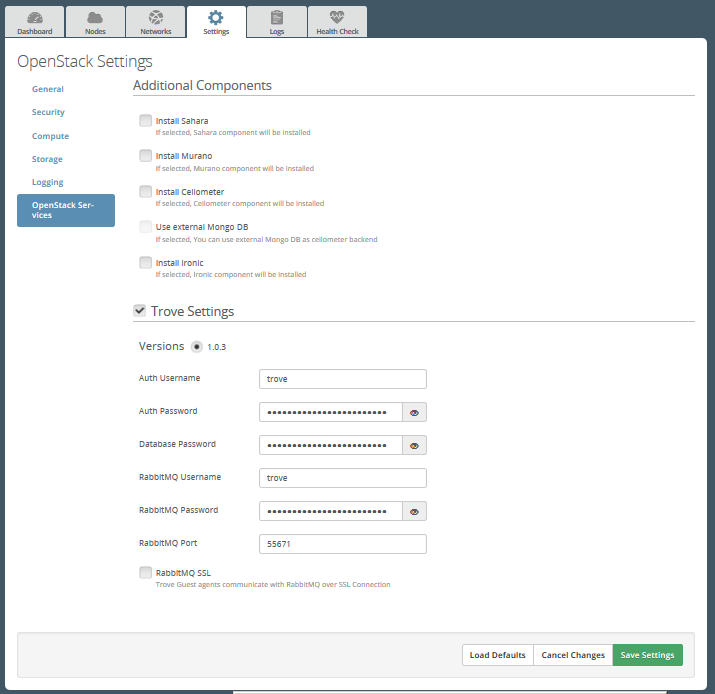
\includegraphics{enable_plugin.png}

\item {} 
Go to the Nodes tab and here push Add Nodes button

\includegraphics{nodes_tab.png}

Note that now Trove role is available in the roles list.

\item {} 
Add nodes to the environment with RabbitMQ role assigned to some of them.
On the screenshot below you may see environment with 1 controller, 1 compute
and one Trove node. You can assign Trove role to more than one
node.

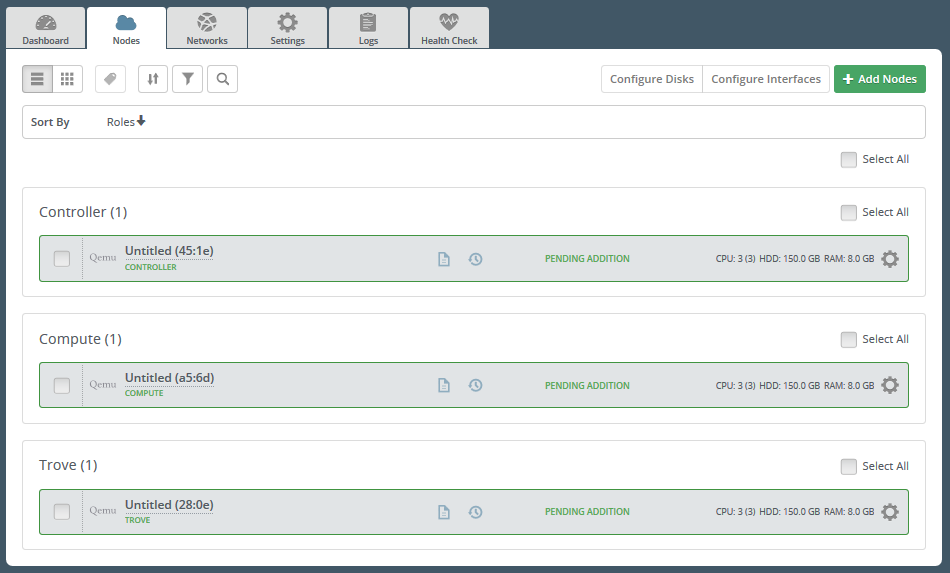
\includegraphics{env_nodes.png}

\item {} 
Finish \href{http://docs.mirantis.com/openstack/fuel/fuel-8.0/fuel-user-guide.html\#configure-your-environment}{configuring your environment} \footnote{
\href{http://docs.mirantis.com/openstack/fuel/fuel-8.0/fuel-user-guide.html\#configure-your-environment}{http://docs.mirantis.com/openstack/fuel/fuel-8.0/fuel-user-guide.html\#configure-your-environment}
}.

\item {} 
\href{http://docs.mirantis.com/openstack/fuel/fuel-8.0/fuel-user-guide.html\#deploy-changes}{Deploy your environment} \footnote{
\href{http://docs.mirantis.com/openstack/fuel/fuel-8.0/fuel-user-guide.html\#deploy-changes}{http://docs.mirantis.com/openstack/fuel/fuel-8.0/fuel-user-guide.html\#deploy-changes}
}.

\end{enumerate}


\section{How it works}
\label{user_guide:how-it-works}
With the plugin enabled, Fuel deployes RabbitMQ and Trove Services on Trove
nodes and here RabbitMQ is also managed by Pacemaker. Also note that two
separate Pacemaker clusters are running on Controller and Trove nodes and
they are not aware of each other.
\begin{description}
\item[{The Trove service logs could be found at :}] \leavevmode\begin{itemize}
\item {} 
on Trove node in /var/log/trove directory

\end{itemize}

\item[{When the plugin is enabled, RabbitMQ log could be found in its regular place:}] \leavevmode\begin{itemize}
\item {} 
on RabbitMQ node in /var/log/rabbitmq directory

\item {} 
on master node in /var/log/remote/\textless{}node-name\textgreater{}/rabbitmq-*.log files

\end{itemize}

\item[{The same applies to log of Pacemaker which manages RabbitMQ. Its location is:}] \leavevmode\begin{itemize}
\item {} 
on RabbitMQ node /var/log/pacemaker.log

\item {} 
on master node in the following files:
\begin{itemize}
\item {} 
/var/log/remote/\textless{}node-name\textgreater{}/attrd.log

\item {} 
/var/log/remote/\textless{}node-name\textgreater{}/crmd.log

\item {} 
/var/log/remote/\textless{}node-name\textgreater{}/cib.log

\item {} 
/var/log/remote/\textless{}node-name\textgreater{}/lrmd.log

\item {} 
/var/log/remote/\textless{}node-name\textgreater{}/pengine.log

\end{itemize}

\end{itemize}

\end{description}


\chapter{Indices and tables}
\label{index:indices-and-tables}\label{index:deploy-your-environment}\begin{itemize}
\item {} 
\emph{genindex}

\item {} 
\emph{modindex}

\item {} 
\emph{search}

\end{itemize}



\renewcommand{\indexname}{Index}
\printindex
\end{document}
